% Supporting Information for the JIFMA manuscript (separate file). Same macros and generated tables as the main document; anonymous.
\documentclass[12pt]{article}
\usepackage[margin=1in]{geometry}\usepackage{mathptmx}\usepackage{setspace}\onehalfspacing
\usepackage{booktabs}\usepackage{array}\usepackage{longtable}\usepackage{amsmath}\usepackage{graphicx}\usepackage{rotating}\usepackage{xr-hyper}\externaldocument{main}\usepackage[hidelinks]{hyperref}\usepackage{apacite}
% generated by code/make_tables_jifma.py on 2026-11-11 (inherits make_tables_cgir.py) — every macro traces to a results file (see the generators for keys)
\newcommand{\NOldN}{464}
\newcommand{\NOldDisposed}{257}
\newcommand{\NOldRetained}{89}
\newcommand{\NOldOther}{43}
\newcommand{\NOldUnresolved}{75}
\newcommand{\NOldPriced}{380}
\newcommand{\NOldPricedOneY}{366}
\newcommand{\NOldOwnership}{387}
\newcommand{\NNewN}{294}
\newcommand{\NNewDisposed}{145}
\newcommand{\NNewRetained}{90}
\newcommand{\NNewOther}{29}
\newcommand{\NNewUnresolved}{30}
\newcommand{\NNewPriced}{260}
\newcommand{\NNewPricedOneY}{249}
\newcommand{\NNewOwnership}{283}
\newcommand{\NAllN}{758}
\newcommand{\NAllDisposed}{402}
\newcommand{\NAllRetained}{179}
\newcommand{\NAllOther}{72}
\newcommand{\NAllUnresolved}{105}
\newcommand{\NAllPriced}{640}
\newcommand{\NAllPricedOneY}{615}
\newcommand{\NAllOwnership}{670}
\newcommand{\NScoreOneY}{559}
\newcommand{\NLabelOneY}{471}
\newcommand{\NGateOne}{579}
\newcommand{\AUCPooledLLM}{0.761}
\newcommand{\AUCPooledFin}{0.587}
\newcommand{\AUCNewLLM}{0.813}
\newcommand{\AUCNewFin}{0.577}
\newcommand{\DeltaPooled}{0.174}
\newcommand{\DeltaPooledLo}{0.117}
\newcommand{\DeltaPooledHi}{0.235}
\newcommand{\AUCOldIdent}{0.706}
\newcommand{\AUCOldAnon}{0.691}
\newcommand{\AUCNewIdent}{0.810}
\newcommand{\AUCNewAnon}{0.803}
\newcommand{\ClaudeOutsideKnowledgeOld}{43.0}
\newcommand{\AUCClaudeFlaggedAnonOld}{0.763}
\newcommand{\AUCClaudeFlaggedIdentOld}{0.764}
\newcommand{\DisposedSharePooled}{69.3}
\newcommand{\GapOldLo}{$-$0.006}
\newcommand{\GapOldHi}{0.039}
\newcommand{\AUCEarlyPooled}{0.780}
\newcommand{\AUCEarlyNew}{0.919}
\newcommand{\AUCEarlyOld}{0.698}
\newcommand{\AUCLateVsNever}{0.708}
\newcommand{\SpearmanAnon}{$-$0.135}
\newcommand{\NAUCEarlyAnon}{339}
\newcommand{\NAUCEarly}{412}
\newcommand{\SpearmanAnonP}{0.001}
\newcommand{\RankAnonCoef}{$-$0.195}
\newcommand{\RankAnonP}{0.005}
\newcommand{\AUCEarlyAnon}{0.817}
\newcommand{\QQDiff}{$-$4.4}
\newcommand{\QQLo}{$-$22.7}
\newcommand{\QQHi}{+17.3}
\newcommand{\QQWithinYear}{$-$11.7}
\newcommand{\QQWithinYearP}{0.154}
\newcommand{\SpearmanScoreBhar}{$-$0.136}
\newcommand{\SpearmanScoreBharP}{0.001}
\newcommand{\SpearmanWithinYear}{$-$0.134}
\newcommand{\SpearmanWithinYearP}{0.002}
\newcommand{\AnnCarSlope}{0.037}
\newcommand{\AnnCarSlopeSE}{0.019}
\newcommand{\AnnCarSlopeP}{0.046}
\newcommand{\CTHiLo}{$-$12.2}
\newcommand{\CTHiLoT}{$-$1.68}
\newcommand{\FFHiLo}{$-$0.52}
\newcommand{\FFHiLoT}{$-$0.96}
\newcommand{\DriftMean}{$-$6.0}
\newcommand{\DriftMedian}{$-$15.9}
\newcommand{\DriftNeg}{66}
\newcommand{\DriftLo}{$-$11.6}
\newcommand{\DriftHi}{$-$0.1}
\newcommand{\AnnCarMean}{+0.58}
\newcommand{\AnnCarT}{1.30}
\newcommand{\AnnCarN}{583}
\newcommand{\FFAllAlpha}{$-$0.02}
\newcommand{\FFAllT}{$-$0.07}
\newcommand{\EarlyN}{195}
\newcommand{\EarlyMean}{$-$14.2}
\newcommand{\EarlyMedian}{$-$26.6}
\newcommand{\NeverN}{141}
\newcommand{\NeverMean}{+1.4}
\newcommand{\NeverMedian}{$-$8.7}
\newcommand{\EarlyNeverDiff}{$-$15.6}
\newcommand{\EarlyNeverLo}{$-$34.2}
\newcommand{\EarlyNeverHi}{+1.3}
\newcommand{\EarlyNeverWelchP}{0.082}
\newcommand{\EarlyNeverMWP}{0.001}
\newcommand{\LateMean}{$-$3.8}
\newcommand{\LateNeverP}{0.626}
\newcommand{\DispRetDiff}{$-$10.3}
\newcommand{\DispRetMWP}{0.010}
\newcommand{\DispRetWelchP}{0.219}
\newcommand{\RankSpecOneCoef}{$-$0.191}
\newcommand{\RankSpecOneP}{0.004}
\newcommand{\RankSpecOneClP}{0.001}
\newcommand{\RankSpecTwoCoef}{$-$0.192}
\newcommand{\RankSpecTwoP}{0.003}
\newcommand{\RankSpecTwoClP}{$<$0.001}
\newcommand{\RankSpecThreeCoef}{$-$0.195}
\newcommand{\RankSpecThreeP}{0.004}
\newcommand{\RankSpecThreeClP}{$<$0.001}
\newcommand{\RankSpecThreeBCoef}{$-$0.229}
\newcommand{\RankSpecThreeBP}{0.019}
\newcommand{\RankSpecThreeBClP}{0.002}
\newcommand{\RankSpecThreeCCoef}{$-$0.168}
\newcommand{\RankSpecThreeCP}{0.097}
\newcommand{\RankSpecThreeCClP}{0.047}
\newcommand{\RankSpecFourCoef}{$-$0.207}
\newcommand{\RankSpecFourP}{0.047}
\newcommand{\RankSpecFourClP}{0.042}
\newcommand{\RankScoreCoefMin}{$-$0.20}
\newcommand{\RankScoreCoefMax}{$-$0.19}
\newcommand{\JointEarlyCoef}{$-$0.151}
\newcommand{\JointEarlyP}{0.083}
\newcommand{\JointScoreCoef}{0.135}
\newcommand{\JointScoreP}{0.549}
\newcommand{\BlockMedian}{34.6}
\newcommand{\LargestMedian}{21.8}
\newcommand{\NOwnership}{551}
\newcommand{\ScoreOnBlock}{$-$0.113}
\newcommand{\ScoreOnBlockP}{0.013}
\newcommand{\ScoreOnBlockClP}{0.004}
\newcommand{\LowBlockDisp}{74}
\newcommand{\HighBlockDisp}{62}
\newcommand{\LowBlockEarly}{52}
\newcommand{\HighBlockEarly}{43}
\newcommand{\LowBlockMedian}{$-$26.9}
\newcommand{\HighBlockMedian}{$-$9.1}
\newcommand{\LowBlockMean}{$-$13.7}
\newcommand{\HighBlockMean}{$-$0.5}
\newcommand{\LowHighMWP}{$<$0.001}
\newcommand{\LowHighDiff}{$-$13.1}
\newcommand{\LowBlockMax}{27}
\newcommand{\HighBlockMin}{43}
\newcommand{\RankOnBlock}{0.14}
\newcommand{\RankOnBlockP}{0.062}
\newcommand{\ProtectPre}{0.5}
\newcommand{\ProtectPost}{95.5}
\newcommand{\ListingPre}{9.1}
\newcommand{\ListingPost}{77.3}
\newcommand{\CarPre}{+0.06}
\newcommand{\CarPost}{+5.29}
\newcommand{\CarPrePostP}{$<$0.001}
\newcommand{\ScorePre}{0.528}
\newcommand{\ScorePost}{0.510}
\newcommand{\ScorePrePostP}{0.616}
\newcommand{\EarlyPre}{40.2}
\newcommand{\NPostOutcomes}{19}
\newcommand{\EarlyPost}{36.8}
\newcommand{\EarlyPrePostP}{1.000}
\newcommand{\NPost}{49}
\newcommand{\NPostFilings}{44}
\newcommand{\FilingsPerYearPre}{39.0}
\newcommand{\FilingsPerYearPost}{16.4}
\newcommand{\NDefs}{10}
\newcommand{\IPOShare}{3.3}
\newcommand{\NClean}{581}
\newcommand{\KLAnnCar}{0.853}
\newcommand{\KLBhar}{$-$10.995}
\newcommand{\KLCar}{$-$7.857}
\newcommand{\KLDisposed}{69.3}
\newcommand{\KLN}{525}
\newcommand{\KLOwnMedian}{14.71}
\newcommand{\KLOwnMean}{18.432}
\newcommand{\RepeatCorrA}{0.96}
\newcommand{\RepeatCorrB}{0.99}
\newcommand{\BetweenModelCorr}{0.87}
\newcommand{\NRepeat}{245}
\newcommand{\KRXCompustatCorr}{0.9998}
\newcommand{\NPriceOverlap}{233}
\newcommand{\GlitchExcluded}{14}
\newcommand{\OwnPairs}{357}
\newcommand{\OwnWithinOne}{354}
\newcommand{\OwnDisagree}{3}
\newcommand{\AUCTemporalFin}{0.611}
\newcommand{\AUCTemporalLLM}{0.813}
\newcommand{\AnnCarSlopePP}{3.7}
\newcommand{\RankSpecThreePctl}{19.5}
\newcommand{\GPTOutsideKnowledgeOld}{3.8}
\newcommand{\CleanDisposedShare}{69.2}
\newcommand{\KLListed}{4.0}
\newcommand{\BlockOnDisposed}{$-$0.092}
\newcommand{\BlockOnDisposedSE}{0.129}
\newcommand{\BlockOnEarlyAlone}{$-$0.141}
\newcommand{\BlockOnEarlyAloneSE}{0.144}
\newcommand{\BlockOnEarlyWithScore}{0.113}
\newcommand{\BlockOnEarlyWithScoreSE}{0.133}
\newcommand{\ScoreOnEarlyWithBlock}{1.235}
\newcommand{\BlockOnCar}{0.030}
\newcommand{\BlockOnCarSE}{0.023}
\newcommand{\EarlyCoefBhar}{$-$0.243}
\newcommand{\LowBlockCoefBhar}{$-$0.231}
\newcommand{\InterCoefBhar}{0.223}
\newcommand{\InterPBhar}{0.114}
\newcommand{\EarlyCoefRank}{$-$0.136}
\newcommand{\LowBlockCoefRank}{$-$0.111}
\newcommand{\InterCoefRank}{0.114}
\newcommand{\InterPRank}{0.071}
\newcommand{\EarlyInLowBlockRank}{$-$0.022}
\newcommand{\LGScore}{0.76}
\newcommand{\LGAnnCar}{$-$7.3}
\newcommand{\LGBhar}{$-$15.3}
\newcommand{\KLKrxTotal}{948}
\newcommand{\KLKrxCaptive}{719}
\newcommand{\NScored}{720}
\newcommand{\QOneMedian}{$-$3.0}
\newcommand{\QFiveMedian}{$-$23.0}
\newcommand{\QQMedianDiff}{$-$20.0}
\newcommand{\QQMWP}{0.008}
\newcommand{\KLLGDrop}{30}
\newcommand{\NSensitive}{11}
\newcommand{\NMixed}{4}
\newcommand{\ExDoosanScore}{0.98}
\newcommand{\ExDoosanOutcome}{disposed}
\newcommand{\ExDBScore}{0.24}
\newcommand{\ExDBOutcome}{retained}
\newcommand{\ExTvingScore}{0.85}
\newcommand{\ExTvingOutcome}{disposed}
\newcommand{\NUnread}{38}
\newcommand{\NUnreadTooRecent}{15}
\newcommand{\NUnreadUnmatched}{13}
\newcommand{\NUnreadMergedLiq}{9}
\newcommand{\NUnreadClean}{1}
\newcommand{\NPostAll}{66}
\newcommand{\KLBharOne}{$-$11.0}
\newcommand{\KLOwnMeanOne}{18.4}
\newcommand{\KLOwnMedianOne}{14.7}
\newcommand{\MDEEarlyPP}{34}
\newcommand{\MDEScore}{0.10}
\newcommand{\ScoreSDPre}{0.22}
\newcommand{\NestedMZero}{0.587}
\newcommand{\NestedMZeroOld}{0.445}
\newcommand{\NestedMZeroNew}{0.581}
\newcommand{\NestedMOne}{0.667}
\newcommand{\NestedMOneOld}{0.566}
\newcommand{\NestedMOneNew}{0.668}
\newcommand{\NestedMTwo}{0.680}
\newcommand{\NestedMTwoOld}{0.599}
\newcommand{\NestedMTwoNew}{0.733}
\newcommand{\NestedMThree}{0.770}
\newcommand{\NestedMThreeOld}{0.706}
\newcommand{\NestedMThreeNew}{0.830}
\newcommand{\NestedF}{0.611}
\newcommand{\NestedFOld}{0.593}
\newcommand{\NestedFNew}{0.689}
\newcommand{\NestedKOne}{0.590}
\newcommand{\NestedKOneOld}{0.521}
\newcommand{\NestedKOneNew}{0.600}
\newcommand{\NestedS}{0.758}
\newcommand{\NestedSOld}{0.700}
\newcommand{\NestedSNew}{0.809}
\newcommand{\NestedIncMThreeMTwo}{+0.09}
\newcommand{\NestedIncMThreeMTwoLo}{0.05}
\newcommand{\NestedIncMThreeMTwoHi}{0.13}
\newcommand{\NestedIncMOneMZero}{+0.08}
\newcommand{\NestedIncKOneMZero}{+0.003}
\newcommand{\NestedIncMThreeMZero}{+0.18}
\newcommand{\NestedLRpMThree}{$<$0.001}
\newcommand{\DecompRTwo}{0.44}
\newcommand{\DecompAUCFitted}{0.675}
\newcommand{\DecompAUCResid}{0.722}
\newcommand{\DecompSaleCoef}{0.32}
\newcommand{\DecompFundCoef}{0.08}
\newcommand{\DecompInvestorCoef}{0.042}
\newcommand{\RankSPlusPurpose}{$-$0.285}
\newcommand{\RankSPlusPurposeP}{0.001}
\newcommand{\RankSPlusPurposeMentions}{$-$0.296}
\newcommand{\RankSPlusPurposeMentionsP}{$<$0.001}
\newcommand{\AnnSPlusPurposeMentions}{0.037}
\newcommand{\AnnSPlusPurposeMentionsP}{0.121}
\newcommand{\PermAUCMin}{0.48}
\newcommand{\PermAUCMax}{0.51}
\newcommand{\CoxN}{484}
\newcommand{\CoxEvents}{324}
\newcommand{\CoxConcordance}{0.73}
\newcommand{\CoxHRSD}{1.96}
\newcommand{\CoxHRSDLo}{1.74}
\newcommand{\CoxHRSDHi}{2.19}
\newcommand{\CoxHRUnit}{36.7}
\newcommand{\CoxHRBlock}{0.964}
\newcommand{\CoxHRBlockLo}{0.908}
\newcommand{\CoxHRBlockHi}{1.024}
\newcommand{\KMLowOneY}{24}
\newcommand{\KMMidOneY}{54}
\newcommand{\KMHighOneY}{74}
\newcommand{\KMAllOneY}{51}
\newcommand{\KMAllFiveY}{68}
\newcommand{\CoxPermHR}{1.22}
\newcommand{\CoxPHp}{0.054}
\newcommand{\RankSSector}{$-$0.194}
\newcommand{\RankSSectorPFirm}{0.004}
\newcommand{\RankSSectorPTwoway}{$<$0.001}
\newcommand{\RankSSic}{$-$0.153}
\newcommand{\RankSGind}{$-$0.167}
\newcommand{\RankSForeign}{$-$0.211}
\newcommand{\RankSForeignP}{0.002}
\newcommand{\RankSForeignN}{540}
\newcommand{\RankSBoard}{$-$0.187}
\newcommand{\RankSBoardP}{0.119}
\newcommand{\RankSBoardN}{194}
\newcommand{\AnnSSector}{0.045}
\newcommand{\AnnSSectorP}{0.020}
\newcommand{\ForeignCoverage}{577}
\newcommand{\ForeignMedian}{2.5}
\newcommand{\BoardN}{211}
\newcommand{\BoardMedian}{0.25}
\newcommand{\EarlySector}{$-$0.077}
\newcommand{\EarlySectorP}{0.013}
\newcommand{\BenchMarketAdjustedPaperRank}{$-$0.195}
\newcommand{\BenchMarketAdjustedPaperRankP}{0.004}
\newcommand{\BenchMarketAdjustedPaperMean}{$-$5.6}
\newcommand{\BenchMarketAdjustedPaperRho}{$-$0.137}
\newcommand{\BenchMarketAdjustedPaperN}{559}
\newcommand{\BenchPfSizebmWithSizeFallbackRank}{$-$0.147}
\newcommand{\BenchPfSizebmWithSizeFallbackRankP}{0.031}
\newcommand{\BenchPfSizebmWithSizeFallbackMean}{$-$8.2}
\newcommand{\BenchPfSizebmWithSizeFallbackRho}{$-$0.090}
\newcommand{\BenchPfSizebmWithSizeFallbackN}{540}
\newcommand{\BenchPfStrictRank}{$-$0.117}
\newcommand{\BenchPfStrictRankP}{0.095}
\newcommand{\BenchPfStrictMean}{$-$7.7}
\newcommand{\BenchPfStrictRho}{$-$0.073}
\newcommand{\BenchPfStrictN}{513}
\newcommand{\BenchPfRank}{$-$0.164}
\newcommand{\BenchPfRankP}{0.019}
\newcommand{\BenchPfMean}{$-$8.1}
\newcommand{\BenchPfRho}{$-$0.085}
\newcommand{\BenchPfN}{513}
\newcommand{\BenchMatchedFirmSizebmRank}{$-$0.017}
\newcommand{\BenchMatchedFirmSizebmRankP}{0.820}
\newcommand{\BenchMatchedFirmSizebmMean}{$-$8.6}
\newcommand{\BenchMatchedFirmSizebmRho}{$-$0.026}
\newcommand{\BenchMatchedFirmSizebmN}{504}
\newcommand{\BenchPsmControlFirmRank}{$-$0.124}
\newcommand{\BenchPsmControlFirmRankP}{0.071}
\newcommand{\BenchPsmControlFirmMean}{$-$3.6}
\newcommand{\BenchPsmControlFirmRho}{$-$0.088}
\newcommand{\BenchPsmControlFirmN}{522}
\newcommand{\SelFirmYears}{43,000}
\newcommand{\SelEvents}{615}
\newcommand{\SelFirms}{3,132}
\newcommand{\SelPseudoR}{0.061}
\newcommand{\SelLogAt}{0.231}
\newcommand{\SelLogAtP}{$<$0.001}
\newcommand{\SelLev}{0.627}
\newcommand{\SelLevP}{0.010}
\newcommand{\SelCf}{$-$2.963}
\newcommand{\SelCfP}{$<$0.001}
\newcommand{\SelSg}{0.186}
\newcommand{\SelSgP}{0.002}
\newcommand{\SelKosdaq}{$-$0.067}
\newcommand{\SelKosdaqP}{0.551}
\newcommand{\SelQ}{0.065}
\newcommand{\SelQP}{0.125}
\newcommand{\SelInv}{0.423}
\newcommand{\SelInvP}{0.609}
\newcommand{\SelCash}{$-$0.344}
\newcommand{\SelCashP}{0.324}
\newcommand{\SelPSAUC}{0.72}
\newcommand{\SelSupport}{100}
\newcommand{\BlockScoreSector}{$-$0.095}
\newcommand{\BlockScoreSectorP}{0.041}
\newcommand{\BlockScoreForeign}{$-$0.143}
\newcommand{\BlockScoreForeignP}{0.002}
\newcommand{\BlockScoreBoard}{$-$0.217}
\newcommand{\BlockScoreBoardP}{0.018}
\newcommand{\BlockScoreBoardN}{191}
\newcommand{\ForeignOnScore}{$-$0.222}
\newcommand{\ForeignOnScoreP}{0.016}
\newcommand{\DiDCxP}{5.45}
\newcommand{\DiDCxPSE}{1.59}
\newcommand{\DiDCxPP}{0.001}
\newcommand{\DiDN}{279}
\newcommand{\DiDNCaptive}{230}
\newcommand{\DiDNEquity}{49}
\newcommand{\DiDNPost}{65}
\newcommand{\DiDCxPLong}{6.52}
\newcommand{\DiDCxPLongP}{$<$0.001}
\newcommand{\DiDPlacebo}{2.27}
\newcommand{\DiDPlaceboP}{0.435}
\newcommand{\DiDCxPTwentyOne}{2.11}
\newcommand{\DiDCxPTwentyOneP}{0.661}
\newcommand{\CarCaptivePre}{$-$0.09}
\newcommand{\CarCaptivePost}{5.51}
\newcommand{\CarEquityPre}{$-$0.28}
\newcommand{\CarEquityPost}{$-$1.30}
\newcommand{\NEquityPost}{24}
\newcommand{\NCaptivePost}{51}
\newcommand{\AppraisalPrices}{40}
\newcommand{\AppraisalProxyDiff}{0.8}
\newcommand{\MoneynessMedian}{1.6}
\newcommand{\MoneynessITM}{60}
\newcommand{\MoneynessQOne}{$-$4.0}
\newcommand{\MoneynessQThree}{4.5}
\newcommand{\PutSlopeTwentyOne}{0.45}
\newcommand{\PutSlopeTwentyOneP}{0.015}
\newcommand{\PutSlopeTwentyOneN}{25}
\newcommand{\PutSlopeThree}{0.39}
\newcommand{\PutSlopeThreeP}{0.172}
\newcommand{\PutSlopeThreeN}{33}
\newcommand{\PutPlaceboPre}{$-$0.074}
\newcommand{\PutPlaceboPreP}{0.072}
\newcommand{\ExerciseMinusHold}{1.1}
\newcommand{\ExerciseBeats}{51}
\newcommand{\ExerciseN}{35}
\newcommand{\ProtPostWithBlock}{61}
\newcommand{\ProtPostN}{66}
\newcommand{\ProtPreWithBlock}{0}
\newcommand{\ProtPreN}{228}
\newcommand{\ProtCharterVote}{7}
\newcommand{\ProtNoListingHorizon}{3}
\newcommand{\ProtSalePlan}{4}
\newcommand{\ProtUnlistedSoft}{32}
\newcommand{\ProtNone}{15}
\newcommand{\ProtStrengthRho}{$-$0.27}
\newcommand{\ProtStrengthP}{0.075}
\newcommand{\ProtDisposedStrengthZero}{62}
\newcommand{\ProtDisposedStrengthOne}{17}
\newcommand{\ProtNLabStrengthZero}{13}
\newcommand{\ProtNLabStrengthOne}{23}
\newcommand{\ProtMeanSNone}{0.68}
\newcommand{\ProtMeanSCharter}{0.50}
\newcommand{\ProtMeanSUnlisted}{0.45}
\newcommand{\ProtMeanSHorizon}{0.34}
\newcommand{\ValN}{579}
\newcommand{\ValAUCId}{0.758}
\newcommand{\ValAUCAn}{0.751}
\newcommand{\ValDAUC}{0.007}
\newcommand{\ValDAUCLo}{$-$0.007}
\newcommand{\ValDAUCHi}{0.021}
\newcommand{\ValDAUCMaxSub}{0.022}
\newcommand{\ValOutsideA}{42}
\newcommand{\ValOutsideB}{4}
\newcommand{\ValSubsetN}{239}
\newcommand{\ValSubsetAUCId}{0.784}
\newcommand{\ValSubsetAUCAn}{0.780}
\newcommand{\ValSubsetDAUC}{0.003}
\newcommand{\ValSubsetLo}{$-$0.035}
\newcommand{\ValSubsetHi}{0.038}
\newcommand{\ValAUCPeriodEarly}{0.64}
\newcommand{\ValGapPeriodEarly}{$-$0.23}
\newcommand{\ValAUCPeriodMiddle}{0.75}
\newcommand{\ValGapPeriodMiddle}{$-$0.22}
\newcommand{\ValAUCPeriodLate}{0.81}
\newcommand{\ValGapPeriodLate}{$-$0.10}
\newcommand{\ValLRDiscPeriod}{0.425}
\newcommand{\ValLRCalPeriod}{0.010}
\newcommand{\ValAUCListedListed}{0.79}
\newcommand{\ValGapListedListed}{$-$0.17}
\newcommand{\ValAUCListedUnlisted}{0.66}
\newcommand{\ValGapListedUnlisted}{$-$0.18}
\newcommand{\ValLRDiscListed}{0.015}
\newcommand{\ValLRCalListed}{0.660}
\newcommand{\ValAUCKosdaqKosdaq}{0.77}
\newcommand{\ValGapKosdaqKosdaq}{$-$0.23}
\newcommand{\ValAUCKosdaqKospiOther}{0.76}
\newcommand{\ValGapKosdaqKospiOther}{$-$0.14}
\newcommand{\ValLRDiscKosdaq}{0.218}
\newcommand{\ValLRCalKosdaq}{0.060}
\newcommand{\ValAUCSizeLarge}{0.82}
\newcommand{\ValGapSizeLarge}{$-$0.03}
\newcommand{\ValAUCSizeMid}{0.85}
\newcommand{\ValGapSizeMid}{$-$0.06}
\newcommand{\ValAUCSizeSmall}{0.63}
\newcommand{\ValGapSizeSmall}{$-$0.27}
\newcommand{\ValLRDiscSize}{0.026}
\newcommand{\ValLRCalSize}{$<$0.001}
\newcommand{\ValAUCMcapLarge}{0.82}
\newcommand{\ValGapMcapLarge}{$-$0.06}
\newcommand{\ValAUCMcapMid}{0.75}
\newcommand{\ValGapMcapMid}{$-$0.17}
\newcommand{\ValAUCMcapSmall}{0.76}
\newcommand{\ValGapMcapSmall}{$-$0.29}
\newcommand{\ValLRDiscMcap}{0.514}
\newcommand{\ValLRCalMcap}{$<$0.001}
\newcommand{\ValAUCForeignHigh}{0.83}
\newcommand{\ValGapForeignHigh}{$-$0.11}
\newcommand{\ValAUCForeignLow}{0.64}
\newcommand{\ValGapForeignLow}{$-$0.24}
\newcommand{\ValAUCForeignMid}{0.79}
\newcommand{\ValGapForeignMid}{$-$0.17}
\newcommand{\ValLRDiscForeign}{0.245}
\newcommand{\ValLRCalForeign}{0.198}
\newcommand{\ValMeanS}{0.52}
\newcommand{\ValMeanY}{0.69}
\newcommand{\ValRecalSlope}{1.46}
\newcommand{\ValStageOneRTwo}{0.53}
\newcommand{\ValMaxBeta}{0.19}
\newcommand{\ValErrSizeBeta}{+0.15}
\newcommand{\ValErrSizeP}{0.005}
\newcommand{\KappaSale}{0.90}
\newcommand{\KappaFund}{0.92}
\newcommand{\KappaHolding}{0.84}
\newcommand{\KappaEff}{0.84}
\newcommand{\KappaBuyer}{0.82}
\newcommand{\KappaAppraisal}{0.76}
\newcommand{\KappaListing}{0.01}
\newcommand{\KappaProtect}{0.24}
\newcommand{\KappaInvestor}{0.46}
\newcommand{\TwoModelCorr}{0.80}
\newcommand{\TwoModelCorrNew}{0.87}
\newcommand{\TwoModelN}{715}
\newcommand{\TwoModelMeanA}{0.59}
\newcommand{\TwoModelMeanB}{0.46}
\newcommand{\WithinModelMinAgree}{0.86}
\newcommand{\KLSale}{12.0}
\newcommand{\KLRetained}{30.7}
\newcommand{\KLSpecial}{89.1}
\newcommand{\KLEff}{5.9}
\newcommand{\OurSaleStrict}{8.5}
\newcommand{\OurSaleBroad}{22.4}
\newcommand{\OurSpecial}{99}
\newcommand{\OurEff}{97}
\newcommand{\OurKLN}{517}
\newcommand{\OurListedShare}{3.9}
\newcommand{\OurRetainedShare}{26.0}
\newcommand{\OurRetainedUpper}{40.3}
\newcommand{\OurOutcomeN}{412}
\newcommand{\RepeatAbsA}{0.04}
\newcommand{\RepeatAbsB}{0.02}
\newcommand{\LabelCrossAgree}{74/85}
\newcommand{\LabelCrossPct}{87.1}
\newcommand{\IndustryParents}{459}
\newcommand{\IndustryEvents}{576}

\newcommand{\tabnote}[1]{\par\vspace{4pt}\begin{minipage}{\linewidth}\singlespacing\small\emph{Note.} #1\end{minipage}}
\newcommand{\captive}{captive spin-off}
\renewcommand{\thetable}{S\arabic{table}}\renewcommand{\thefigure}{S\arabic{figure}}
\title{Supporting Information\\[4pt]\large Controlling Owners, Disclosed Intentions, and Minority Shareholder Returns in Korean Captive Spin-Offs}\author{}\date{}
\begin{document}
\maketitle
\noindent This document contains the exhibits referred to in the main text as Tables S1--S5 and Figures S1--S5, and the full definitions of the measures. All numbers are generated from the same results files as the main text.

\section{Measurement validity and bias of the disposal signal (Table S1)}
\begin{sidewaystable}[htbp]\centering\caption{Validity and bias of the disposal signal}\label{tab:s_validity}
{\scriptsize\setlength{\tabcolsep}{3pt}% generated by code/make_tables_jifma.py on 2026-11-11 — source: results/validity_bias_audit_20261111.json -> A_subgroups, B_anonymization, D_two_model_agreement, E_kang_lee_benchmark
\begin{tabular}{llrccc}
\toprule
\multicolumn{6}{l}{\emph{Panel A. Discrimination and calibration of $S$ by subgroup}} \\
Grouping & Level & $n$ & AUC [95\% CI] & Mean $S$ $-$ realised rate & Brier \\
\midrule
Period & 2001-08 & 161 & 0.639 [0.533, 0.743] & $-$0.230 & 0.220 \\
Period & 2009-16 & 178 & 0.751 [0.661, 0.834] & $-$0.222 & 0.224 \\
Period & 2017+ & 240 & 0.813 [0.760, 0.865] & $-$0.095 & 0.184 \\
\multicolumn{6}{l}{\quad LR tests: calibration (group dummies) $p = 0.010$; discrimination ($S \times$ group) $p = 0.425$} \\
Parent listed & listed & 476 & 0.785 [0.741, 0.827] & $-$0.169 & 0.200 \\
Parent listed & unlisted & 103 & 0.658 [0.539, 0.779] & $-$0.183 & 0.238 \\
\multicolumn{6}{l}{\quad LR tests: calibration (group dummies) $p = 0.660$; discrimination ($S \times$ group) $p = 0.015$} \\
Exchange & KOSDAQ & 200 & 0.767 [0.693, 0.836] & $-$0.226 & 0.219 \\
Exchange & KOSPI/other & 379 & 0.762 [0.709, 0.811] & $-$0.142 & 0.200 \\
\multicolumn{6}{l}{\quad LR tests: calibration (group dummies) $p = 0.060$; discrimination ($S \times$ group) $p = 0.218$} \\
Parent assets tercile (2009+) & large & 112 & 0.823 [0.740, 0.898] & $-$0.032 & 0.167 \\
Parent assets tercile (2009+) & mid & 112 & 0.846 [0.776, 0.914] & $-$0.056 & 0.181 \\
Parent assets tercile (2009+) & small & 112 & 0.631 [0.484, 0.765] & $-$0.271 & 0.232 \\
\multicolumn{6}{l}{\quad LR tests: calibration (group dummies) $p = $<$0.001$; discrimination ($S \times$ group) $p = 0.026$} \\
Market cap tercile (listed) & large & 158 & 0.816 [0.752, 0.880] & $-$0.055 & 0.177 \\
Market cap tercile (listed) & mid & 157 & 0.753 [0.665, 0.831] & $-$0.165 & 0.211 \\
Market cap tercile (listed) & small & 158 & 0.764 [0.669, 0.850] & $-$0.287 & 0.213 \\
\multicolumn{6}{l}{\quad LR tests: calibration (group dummies) $p = $<$0.001$; discrimination ($S \times$ group) $p = 0.514$} \\
Foreign ownership tercile & high & 154 & 0.832 [0.767, 0.890] & $-$0.109 & 0.180 \\
Foreign ownership tercile & low & 153 & 0.642 [0.531, 0.748] & $-$0.240 & 0.218 \\
Foreign ownership tercile & mid & 153 & 0.790 [0.707, 0.865] & $-$0.169 & 0.205 \\
\multicolumn{6}{l}{\quad LR tests: calibration (group dummies) $p = 0.198$; discrimination ($S \times$ group) $p = 0.245$} \\
Filing length tercile & long & 193 & 0.764 [0.699, 0.824] & $-$0.091 & 0.197 \\
Filing length tercile & mid & 193 & 0.804 [0.729, 0.870] & $-$0.199 & 0.205 \\
Filing length tercile & short & 193 & 0.691 [0.602, 0.780] & $-$0.225 & 0.218 \\
\multicolumn{6}{l}{\quad LR tests: calibration (group dummies) $p = 0.025$; discrimination ($S \times$ group) $p = 0.332$} \\
GICS sector & 15 & 58 & 0.803 [0.675, 0.909] & $-$0.082 & 0.183 \\
GICS sector & 20 & 84 & 0.735 [0.620, 0.842] & $-$0.153 & 0.215 \\
GICS sector & 25 & 82 & 0.827 [0.723, 0.914] & $-$0.099 & 0.185 \\
GICS sector & 35 & 37 & 0.815 [0.638, 0.955] & $-$0.166 & 0.201 \\
GICS sector & 45 & 113 & 0.639 [0.519, 0.757] & $-$0.255 & 0.225 \\
GICS sector & 50 & 50 & 0.923 [0.829, 0.988] & $-$0.192 & 0.161 \\
GICS sector & other/small & 155 & 0.731 [0.640, 0.813] & $-$0.187 & 0.224 \\
\multicolumn{6}{l}{\quad LR tests: calibration (group dummies) $p = 0.175$; discrimination ($S \times$ group) $p = 0.068$} \\
\midrule
\multicolumn{6}{l}{\emph{Panel B. Identified vs name-anonymised judgments (paired bootstrap)}} \\
Sample & & $n$ & AUC identified & AUC anonymised & $\Delta$AUC [95\% CI] \\
\midrule
All filings & & 579 & 0.758 & 0.751 & 0.007 [$-$0.007, 0.021] \\
Model A only & & 573 & 0.770 & 0.763 & 0.007 [$-$0.016, 0.029] \\
Model B only & & 579 & 0.734 & 0.729 & 0.004 [$-$0.010, 0.018] \\
Model A, self-reported outside knowledge & & 239 & 0.784 & 0.780 & 0.003 [$-$0.035, 0.038] \\
Model A, no outside knowledge reported & & 334 & 0.761 & 0.749 & 0.012 [$-$0.019, 0.040] \\
Model B, no outside knowledge reported & & 557 & 0.730 & 0.725 & 0.005 [$-$0.009, 0.020] \\
\midrule
\multicolumn{6}{l}{\emph{Panel C. Two-model agreement on extracted facts (identified reading, run 1)}} \\
Field & & $n$ & Prevalence A / B & Agreement & $\kappa$ \\
\midrule
Purpose: sale or disposal & & 715 & 0.10 / 0.08 & 0.983 & 0.90 \\
Purpose: fund-raising / investor & & 715 & 0.18 / 0.16 & 0.978 & 0.92 \\
Purpose: holding-company restructuring & & 715 & 0.17 / 0.14 & 0.958 & 0.84 \\
Purpose: efficiency & & 715 & 0.96 / 0.96 & 0.987 & 0.84 \\
Purpose: specialisation & & 715 & 0.98 / 0.98 & 0.985 & 0.61 \\
Purpose: regulatory / legal & & 715 & 0.04 / 0.04 & 0.989 & 0.85 \\
Purpose: other & & 715 & 0.22 / 0.08 & 0.825 & 0.33 \\
Mentions a sale or buyer & & 715 & 0.10 / 0.12 & 0.964 & 0.82 \\
Mentions an outside investor & & 715 & 0.14 / 0.26 & 0.824 & 0.46 \\
Appraisal-right notice & & 715 & 0.68 / 0.78 & 0.903 & 0.76 \\
Mentions listing / IPO (definition split) & & 715 & 0.08 / 0.94 & 0.140 & 0.01 \\
Mentions protection measures & & 715 & 0.06 / 0.32 & 0.740 & 0.24 \\
\multicolumn{6}{l}{Most-likely path: agreement 0.52, $\kappa = 0.34$; $p$ correlation 0.80 (715 filings)} \\
\midrule
\multicolumn{6}{l}{\emph{Panel D. Kang and Lee (2025b) hand-coded benchmark, listed parents 2001--2021}} \\
Quantity & & K\&L ($n = 525$) & Ours & & \\
\midrule
Purpose: sale & & 12.0\% & 8.5\% strict; 22.4\% incl.\ fund-raising ($n = 517$) & & \\
Purpose: specialisation / efficiency & & 89.1\% / 5.9\% & 99.4\% / 96.9\% (multi-label; not comparable) & & \\
Subsidiary eventually listed & & 4.0\% & 3.9\% ($n = 412$) & & \\
Subsidiary retained & & 30.7\% & 26.0\% at 100\%; 40.3\% incl.\ partial stake sales & & \\
\bottomrule
\end{tabular}
}
\tabnote{Panel A: AUC of the two-model signal against the clean-label disposal indicator within each subgroup of the \ValN{} Gate-1 divisions, with a stratified bootstrap 95 percent interval (2,000 resamples); the gap is the mean signal minus the realised disposal rate; LR tests compare a logit of the outcome on logit($S$) with (i) group dummies added (calibration) and (ii) group $\times$ logit($S$) interactions added (discrimination). Parent assets are the surviving company's total assets stated in the filing (available for 2009 onward); market capitalisation and foreign ownership are for listed parents; GICS sectors from Compustat Global. Panel B: the same filings read with and without the parent's and new company's names, group names, tickers and dates; the difference in AUC is a paired bootstrap over events; the self-reported subset uses the model's own flag for having used knowledge outside the filing. Panel C: Cohen's $\kappa$ between the two models' structured extractions on the identified first run; ``definition split'' marks a field whose boundary the two models interpret differently (Model~B marks the form line ``re-listing application: no'' as a mention of listing), not a reading disagreement. Panel D: \citeA{kang2025}, Table 1, Panel A (525 \captive{}s by KOSPI/KOSDAQ-listed parents, 2001--2021), against the majority-vote extraction on our listed-parent filings of 2001--2021 and our outcome labels on the clean-label listed-parent divisions of the same years.}
\end{sidewaystable}

The anonymised signal reproduces the return results: the Spearman correlation with the one-year market-adjusted return is \SpearmanAnon{} ($p$ = \SpearmanAnonP{}) and the within-year rank coefficient with the full controls \RankAnonCoef{} ($p$ = \RankAnonP{}); the early-disposal AUC is \AUCEarlyAnon{} on the \NAUCEarlyAnon{} events with an anonymised score and a recorded timing. The raw signal under-predicts disposal (mean \ValMeanS{} against \ValMeanY{}); because every test in the paper uses the signal's ordering (AUC, ranks, terciles) or its level with year effects, the under-prediction affects no reported coefficient's sign.

\section{Label definitions and sensitivity (Table S2)}
\begin{table}[htbp]\centering\caption{Headline results with the \NSensitive{} definition-sensitive labels flipped or dropped}\label{tab:s_labels}
{\footnotesize\setlength{\tabcolsep}{3pt}% generated by code/make_tables_cgir.py on 2026-11-14 — source: label_sensitivity_20261025.json
\begin{tabular}{>{\raggedright\arraybackslash}p{6.2cm}rrr}
\toprule
 & Labels as used & Eleven set to retained & Eleven dropped \\
\midrule
Clean-label events with returns & 476 & 476 & 468 \\
Disposed share (\%) & 69.5 & 67.9 & 69.0 \\
AUC, two-model disposal score (pooled; 2017+) & 0.785; 0.830 & 0.790; 0.844 & 0.792; 0.850 \\
Disposed $-$ retained, one-year BHAR (\%) [MW $p$] & $-$10.3 [0.010] & $-$14.6 [0.002] & $-$11.8 [0.006] \\
Early $-$ never, one-year BHAR (\%) [MW $p$] & $-$15.6 [0.001] & $-$18.3 [$<$0.001] & $-$15.6 [0.001] \\
Rank of BHAR on early disposal, controls [HC1 $p$] & $-$0.079 [0.013] & $-$0.079 [0.013] & $-$0.079 [0.013] \\
Disposal rate, low / high block tercile (\%) & 74 / 62 & 72 / 59 & 74 / 61 \\
\bottomrule
\end{tabular}
}\tabnote{\NSensitive{} of the 2017--2026 labels are sensitive to the outcome definition or to a disagreement between the equity-investment schedule and the annual-report text (categories: intragroup transfer, temporary external dilution, related-party preferred shares, dilution below materiality, unresolved conflict, one tracker mismatch). Column 2 recodes all of them as retained, the direction least favourable to the paper's results; column 3 drops them.}\end{table}

\section{Selection into captive spin-offs (Table S3)}
\begin{table}[htbp]\centering\caption{Firm-year logit of the \captive{} decision on the Compustat Global universe}\label{tab:s_selection}
{\footnotesize\setlength{\tabcolsep}{3pt}% generated by code/make_tables_jifma.py on 2026-11-11 — source: results/matched_benchmark_selection_20261110.json -> selection_logit
\begin{tabular}{lcc}
\toprule
Covariate (year $t-1$) & Coefficient (firm-clustered s.e.) & $p$ \\
\midrule
log total assets & 0.231*** (0.038) & $<$0.001 \\
Tobin's $q$ & 0.065 (0.042) & 0.125 \\
Leverage & 0.627** (0.243) & 0.010 \\
Investment / assets & 0.423 (0.827) & 0.609 \\
Cash flow / assets & $-$2.963*** (0.450) & $<$0.001 \\
Cash / assets & $-$0.344 (0.349) & 0.324 \\
Sales growth & 0.186*** (0.060) & 0.002 \\
KOSDAQ & $-$0.067 (0.113) & 0.551 \\
Parent-only accounts & 0.074 (0.109) & 0.500 \\
\midrule
Firm-years / events / firms & \multicolumn{2}{c}{43,000 / 615 / 3,132} \\
Pseudo-$R^2$; AUC of the propensity score & \multicolumn{2}{c}{0.061; 0.72} \\
\bottomrule
\end{tabular}
}\tabnote{Korean common stocks in Compustat Global (consolidated accounts where reported, parent-only otherwise, with an indicator), firm-years 2000--2025; the dependent variable is one in the year a \captive{} is announced. Covariates are lagged one year: log total assets, Tobin's $q$, debt to assets, capital expenditure to assets, operating cash flow to assets, cash to assets, sales growth, KOSDAQ listing. Standard errors clustered by firm. The propensity score from this model selects the control firm of Table~4, Panel C; \SelSupport{} percent of events lie inside the controls' support. Signs agree with the selection model of \citeA{kang2025} (Table 4) on size, leverage, cash flow and investment and differ on the exchange indicator.}\end{table}

\section{Industry fixed effects and clustered inference (Table S4)}
\begin{table}[htbp]\centering\caption{Returns on the disposal signal with alternative fixed effects and clustering}\label{tab:s_industry}
{\footnotesize\setlength{\tabcolsep}{3pt}% generated by code/make_tables_jifma.py on 2026-11-14 — source: results/industry_fe_firm_clusters_20261110.json -> table6_returns_on_signal
\begin{tabular}{lcccc}
\toprule
Outcome and specification & Coefficient on $S$ & $p$ HC1 & $p$ firm cluster & $p$ two-way cluster \\
\midrule
One-year BHAR, within-year rank, year FE & $-$0.195 & 0.004 & 0.003 & $<$0.001 \\
One-year BHAR, within-year rank, year + GICS sector FE & $-$0.194 & 0.006 & 0.004 & $<$0.001 \\
One-year BHAR, within-year rank, year + GICS industry FE & $-$0.167 & 0.025 & 0.015 & 0.001 \\
One-year BHAR, within-year rank, year + 2-digit SIC FE & $-$0.153 & 0.031 & 0.020 & 0.002 \\
One-year BHAR, year FE & $-$0.158 & 0.283 & 0.265 & 0.332 \\
One-year BHAR, year + GICS sector FE & $-$0.166 & 0.269 & 0.249 & 0.289 \\
One-year BHAR, year + GICS industry FE & $-$0.198 & 0.204 & 0.172 & 0.143 \\
One-year BHAR, year + 2-digit SIC FE & $-$0.090 & 0.578 & 0.552 & 0.579 \\
One-year market-model CAR, year FE & $-$0.031 & 0.832 & 0.825 & 0.841 \\
One-year market-model CAR, year + GICS sector FE & $-$0.079 & 0.604 & 0.588 & 0.621 \\
One-year market-model CAR, year + GICS industry FE & $-$0.182 & 0.260 & 0.225 & 0.233 \\
One-year market-model CAR, year + 2-digit SIC FE & 0.004 & 0.978 & 0.977 & 0.977 \\
Three-day announcement CAR, year FE & 0.039 & 0.041 & 0.037 & 0.064 \\
Three-day announcement CAR, year + GICS sector FE & 0.045 & 0.025 & 0.020 & 0.063 \\
Three-day announcement CAR, year + GICS industry FE & 0.037 & 0.097 & 0.065 & 0.113 \\
Three-day announcement CAR, year + 2-digit SIC FE & 0.054 & 0.012 & 0.006 & 0.023 \\
\bottomrule
\end{tabular}
}\tabnote{Coefficient on the two-model signal in the specification of Table~4, column (1), re-estimated with the stated fixed effects (GICS sector, GICS industry and two-digit SIC codes of the parent from Compustat Global, linked by gvkey; current classification) and $p$-values from HC1, parent-clustered and two-way parent-and-year-clustered standard errors. \IndustryEvents{} events of \IndustryParents{} parents.}\end{table}

\section{Comparison with the hand-coded sample of Kang and Lee (Table S5)}
\begin{table}[htbp]\centering\caption{The tests of \protect\citeA{kang2025} and their counterparts in this paper}\label{tab:s_mirror}
{\footnotesize\setlength{\tabcolsep}{3pt}% generated by code/make_tables_cgir.py (labels remapped by make_tables_jifma.py) on 2026-11-11 — source: literature/anchor_numbers.json (Kang & Lee 2025, Table 1 Panel B, Tables 2-3, footnotes 14 and 18, Section 4) and our results files
\begin{tabular}{>{\raggedright\arraybackslash}p{5.2cm}>{\raggedright\arraybackslash}p{4.6cm}>{\raggedright\arraybackslash}p{5.4cm}}
\toprule
Test & \protect\citeA{kang2025}, 525 captive spin-offs 2001--2021 & This paper \\
\midrule
Announcement CAR [$-$1, +1] & 0.853\% ($t$ = 2.31) & +0.58\% ($t$ = 1.3), $n$ = 583 \\
One-year abnormal return after the announcement & CAR[+2, +252] $-$7.857\%; BHAR[+2, +252] $-$10.995\% (matched portfolio) & BHAR[+2, +250] mean $-$6.0\%, median $-$15.9\% (market-adjusted), $n$ = 578 \\
Share of subsidiaries eventually disposed of & 69.3\% (364 of 525) & 69.3\% of 579 clean-label events; listed share 3.3\% of 581 clean labels \\
Long-run return, disposed vs retained & disposed $-$16.7\% to $-$10.45\%; retained slightly positive, insignificant & disposed $-$8.9\% vs retained +1.4\% (Mann--Whitney $p$ 0.010); early disposers $-$14.2\% \\
Controlling ownership and long-run return & below-median ownership $-$19.38\% to $-$12.18\%; above-median $-$2.58\% to $-$1.01\%; coefficient 0.511--0.769 & low tercile median $-$26.9\% vs high $-$9.1\%; rank on block 0.142 ($p$ 0.062) \\
Controlling ownership and announcement CAR & coefficient 0.052** & 0.030 (HC1 $p$ 0.199) \\
Ownership and the retention decision & ownership positively associated with retention (unreported) & disposal rate 74\% (low block) vs 62\% (high); disposal on block $-$0.092 ($p$ 0.474) \\
Can investors discern the intention at the announcement? & stated as unlikely; not tested & tested: the filing predicts disposal (Table~\ref{tab:gate1}); the announcement reaction does not price it (Table~\ref{tab:returns}) \\
\bottomrule
\end{tabular}
}\tabnote{Left column: results as reported by \citeA{kang2025} for \KLN{} \captive{}s announced by listed parents between 2001 and 2021; their long-run abnormal returns use a matched portfolio and their ownership measure is the controlling family's and inside directors' stake. Right column: this paper's counterparts with market-adjusted buy-and-hold returns and the controlling block of the main text. The two samples were built independently from the regulator's filings; Table S1, Panel D, compares the two samples' purpose codes and outcome shares.}\end{table}

\section{Results by period, price and ownership sources}
\begin{table}[htbp]\centering\caption{Headline return results by period}\label{tab:s_period}
{\footnotesize\setlength{\tabcolsep}{3pt}% generated by code/make_tables_cgir.py on 2026-11-14 — source: bhar_predicted_disposal_pooled_20261028.json by_period
\begin{tabular}{lrrrr}
\toprule
Period & $n$ & Q5 $-$ Q1 BHAR (\%) [CI] & Spearman $\rho$ [$p$] & CAR slope [$p$] \\
\midrule
2001--2016 & 350 & $-$14.4 [$-$33.0, +6.6] & $-$0.177 [0.001] & 0.0588 [0.070] \\
2017--2026 & 209 & $-$5.6 [$-$29.0, +14.5] & $-$0.074 [0.290] & 0.0192 [0.361] \\
\bottomrule
\end{tabular}
}\tabnote{Listed parents with a disposal signal and a full one-year window, by announcement period. Q5 $-$ Q1 is the mean one-year market-adjusted BHAR difference between the top and bottom quintiles of the signal with a bootstrap 95 percent interval; Spearman correlation between the signal and the one-year BHAR; CAR slope is the OLS coefficient of the three-day announcement CAR on the signal with year fixed effects (HC1 $p$).}\end{table}
\begin{table}[htbp]\centering\caption{Two price sources: cross-check and screen}\label{tab:s_prices}
{\footnotesize\setlength{\tabcolsep}{3pt}% generated by code/make_tables_cgir.py on 2026-11-14 — source: price_coverage_compustat_20261024.json; bhar_pooled_glitch_screen_20261028.json
\begin{tabular}{>{\raggedright\arraybackslash}p{11cm}r}
\toprule
Price-source cross-check and screen & \\
\midrule
2017+ events priced in both sources & 233 \\
Trading days compared & 110,420 \\
Median correlation of daily returns & 0.9998 \\
Share of days on which the two sources differ by more than 1 pp (\%) & 0.2 \\
Share of events with correlation below 0.95 (\%) & 2.1 \\
\midrule
2001--2016 priced events & 380 \\
\quad with a day beyond the exchange price limit in [$-$1, +250] & 26 \\
\quad of which in delisting proceedings (kept) & 12 \\
\quad suspected adjustment errors (excluded) & 14 \\
\bottomrule
\end{tabular}
}\tabnote{Daily adjusted prices from the Korea Exchange (2017--2026) and Compustat Global (2001--2016). Returns are compared on the events priced in both sources over trading days $-250$ to $+250$. The screen flags a 2001--2016 event when a daily return in $[-1, +250]$ exceeds the exchange's daily price limit by more than one percentage point; flagged events whose parent was in delisting proceedings are kept, the rest are excluded from the main results and included in a sensitivity run.}\end{table}
\begin{table}[htbp]\centering\caption{Pre-announcement ownership: two sources and their agreement}\label{tab:s_ownership}
{\footnotesize\setlength{\tabcolsep}{3pt}% generated by code/make_tables_cgir.py on 2026-11-11 — source: largest_shareholder_coverage_20261025.json; ownership_llm_agreement_20261025.json
\begin{tabular}{>{\raggedright\arraybackslash}p{6.6cm}>{\raggedright\arraybackslash}p{3.2cm}>{\raggedright\arraybackslash}p{4.2cm}}
\toprule
Pre-announcement ownership of the parent & DART table (2016+) & Annual-report extraction (pre-2016) \\
\midrule
Events with a usable record & 326 & 373 passages; 357 with figures \\
Median controlling block (\%) & 36.0 & see the main text (block terciles) \\
Two-extractor agreement: largest holder within 0.5 pp & -- & 355 / 357 \\
Two-extractor agreement: block within 1 pp & -- & 354 / 357 \\
Records excluded for internal or cross-extractor disagreement & 5 & 3 \\
\bottomrule
\end{tabular}
}\tabnote{The controlling block is the largest shareholder's and related parties' common shares, excluding treasury shares, at the fiscal year-end before the announcement year. For announcements from 2016 the figure is read from the largest-shareholder table returned by the regulator's interface; for earlier announcements the same table is read from the annual report's text by two language models independently, and a record is kept when the two agree within one percentage point.}\end{table}

\section{Additional figures}
\begin{figure}[htbp]\centering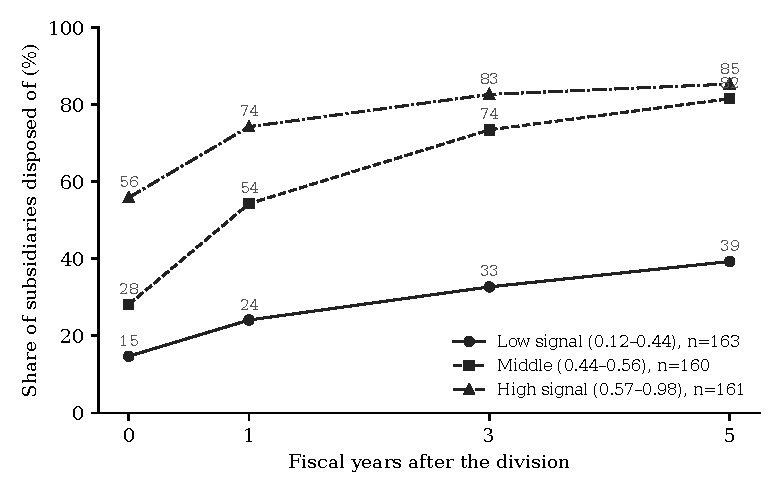
\includegraphics[width=0.8\textwidth]{../figures/F7_km_signal.pdf}\caption{Share of subsidiaries disposed of, by tercile of the disposal signal}\tabnote{Kaplan--Meier cumulative shares from Table 4, Panel B of the main text, at the end of fiscal years 0, 1, 3 and 5 after the division, by tercile of the two-model signal (ranges in the legend); \CoxN{} divisions with a recorded disposal year or a censoring year.}\end{figure}
\begin{figure}[htbp]\centering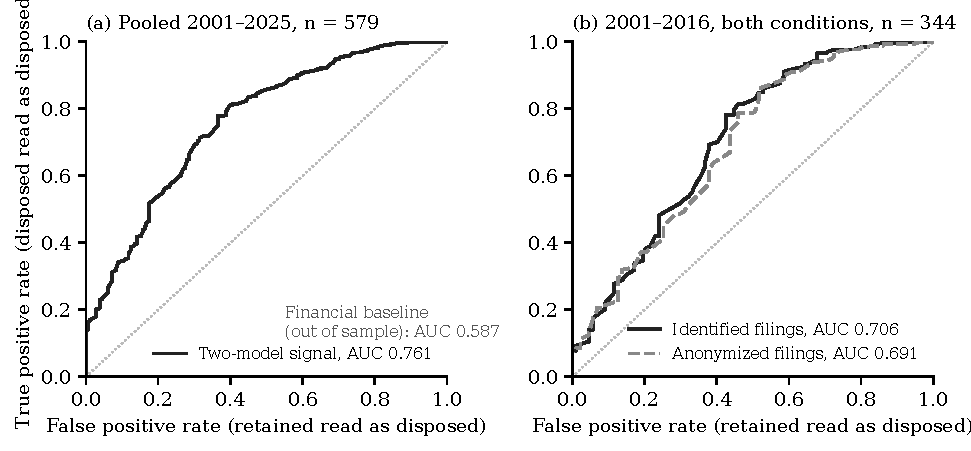
\includegraphics[width=0.97\textwidth]{../figures/F5_roc.pdf}\caption{Receiver operating characteristic curves of the disposal signal}\tabnote{Panel (a): the pooled Gate-1 sample with the out-of-sample AUC of the financial baseline for comparison. Panel (b): the 2001--2016 divisions read in the identified and the anonymised condition.}\end{figure}
\begin{figure}[htbp]\centering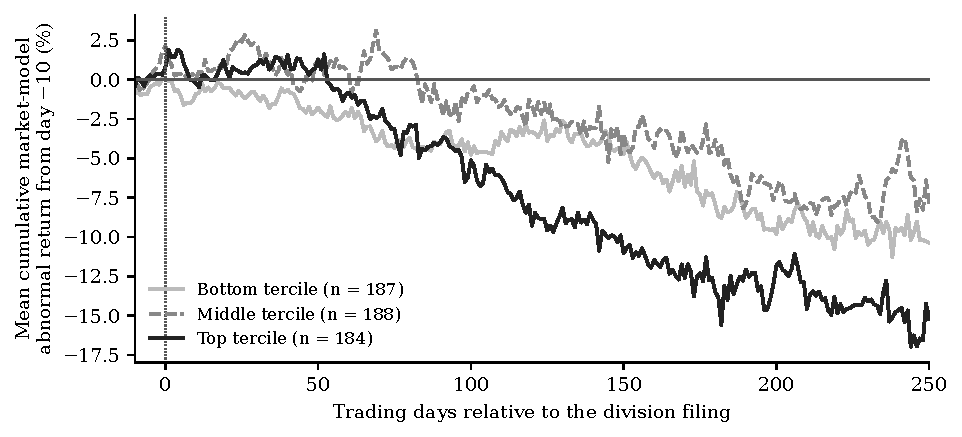
\includegraphics[width=\textwidth]{../figures/F3_car_paths.pdf}\caption{Cumulative abnormal return paths by tercile of the disposal signal}\tabnote{Mean cumulative market-model abnormal return from trading day $-10$, by tercile of the disposal signal, for the listed parents with a full one-year window; day 0 is the first trading day on or after the filing.}\end{figure}
\begin{figure}[htbp]\centering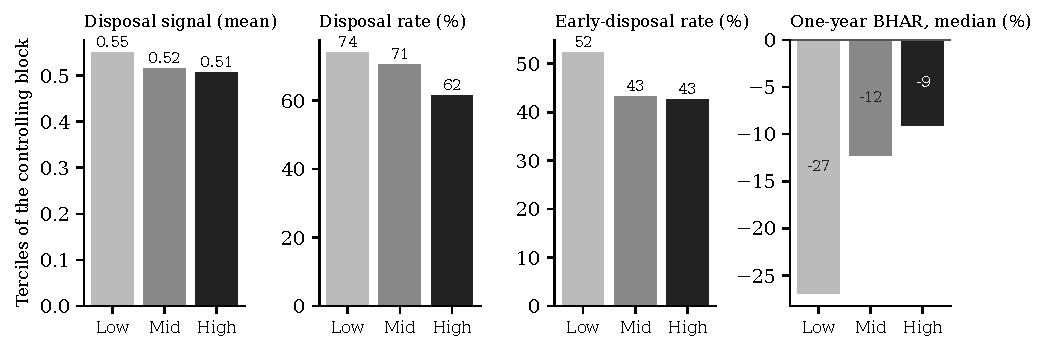
\includegraphics[width=\textwidth]{../figures/F6_block.pdf}\caption{Signal, disposal and returns by tercile of the controlling block}\tabnote{By tercile of the controlling block held before the announcement (low: up to \LowBlockMax{} percent of common shares; high: \HighBlockMin{} percent and above): mean disposal signal, disposal rate on clean labels, early-disposal rate on the subset with a recorded timing, and the median one-year market-adjusted BHAR.}\end{figure}
\begin{figure}[htbp]\centering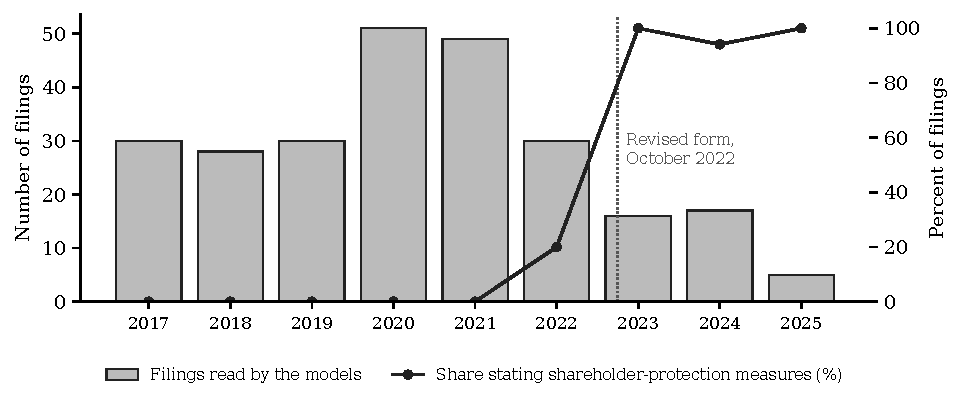
\includegraphics[width=\textwidth]{../figures/F4_reform.pdf}\caption{Captive spin-off filings and shareholder-protection statements by year, 2017--2025}\tabnote{Bars: filings read by the two models in each year; line: share of those filings in which the majority of model judgments flag a shareholder-protection statement. The dotted line marks October 2022, when the revised disclosure form took effect.}\end{figure}

\section{Definitions in full}
{\footnotesize% generated by code/make_tables_cgir.py (labels remapped by make_tables_jifma.py) on 2026-11-14 — source: DEFS list in code/make_tables_cgir.py (same rows as T_defs_short)
\begin{longtable}{>{\raggedright\arraybackslash}p{0.7cm}>{\raggedright\arraybackslash}p{2.4cm}>{\raggedright\arraybackslash}p{3.5cm}>{\raggedright\arraybackslash}p{4.8cm}>{\raggedright\arraybackslash}p{2.1cm}}
\caption{Definitions of the measures used in this paper (full form)}\label{tab:s_defs_full}\\
\toprule No. & Term & Conceptual definition & Operational rule and source & Applied in \\ \midrule \endfirsthead
\multicolumn{5}{l}{\small Table~\thetable\ (continued)}\\ \toprule No. & Term & Conceptual definition & Operational rule and source & Applied in \\ \midrule \endhead
\midrule\multicolumn{5}{r}{\small continued on next page}\\ \endfoot
\bottomrule \endlastfoot
D1 & Captive spin-off (\emph{mulchŏk bunhal}) & A corporate division under the Korean Commercial Act's division provisions in which the surviving company holds 100\% of the newly created company \protect\cite{kang2025}; unlike a US spin-off no shares are distributed to the parent's shareholders, and unlike an equity carve-out no shares are sold or listed at the division. & DART division-resolution filings (\emph{hoesa bunhal gyeoljeong}; from 2017 the material-event report) whose division type is the captive form (a mixed captive--equity division is kept when a wholly owned company is created); author rule, Section~\ref{sec:sample}. & Table~\ref{tab:sample}; all tests \\ \addlinespace[2pt]
D2 & Disposal & The event through which the value of the carved-out assets leaves the parent's minority shareholders \protect\cite{kang2025}: a sale, a listing, or a dilution of the parent's stake. & Ownership of the new company read from the parent's annual reports (the schedule of equity investments in other corporations and the notes on subsidiaries) for each fiscal year from the division to 2025, with KIND listing records; majority sale, listing, or stake below 99.5\% = disposed; 100\% throughout = retained; mergers back into the parent and liquidations excluded; author rule, Section~\ref{sec:sample}. & Tables~\ref{tab:sample}, \ref{tab:gate1}, \ref{tab:returns} \\ \addlinespace[2pt]
D3 & Early disposal & Disposal within the one-year return window. & first\_change\_fy $-$ division year $\le 1$ from the annual-report labels; author rule. & Tables~\ref{tab:returns}, \ref{tab:block} \\ \addlinespace[2pt]
D4 & Disposal signal & What a careful reader could infer about the controlling owner's intention from the filing alone at the announcement (\protect\citeNP{kang2025}, Section 4, call this unlikely). & Each model reads the division-resolution filing as of its date and returns a probability (0--100) that the parent will not retain 100\% within three to five fiscal years; mean over runs per model, then the two-model mean; identified condition unless stated; Section~\ref{sec:signal}. & Tables~\ref{tab:gate1}, \ref{tab:returns} \\ \addlinespace[2pt]
D5 & Anonymised condition & A reading that cannot use knowledge of the named company's later history \protect\cite{glasserman2024}. & Regular-expression masking of names, group names and dates before the model reads the text; Section~\ref{sec:signal}. & Table~\ref{tab:gate1} \\ \addlinespace[2pt]
D6 & Controlling block & The controlling owner's cash-flow stake in the parent, the quantity that determines how much of a minority loss the controller bears \protect\cite{young2008}. & 2016+ announcements: the largest-shareholder table of the annual report via the DART API, total row minus treasury-share rows; earlier: the same table read from the annual report of the pre-division fiscal year (year-end column), or of the division year (year-start column) when the former is not available; Section~\ref{sec:returns}. & Table~\ref{tab:block} \\ \addlinespace[2pt]
D7 & Announcement CAR & The immediate price reaction to the filing. & Market model estimated on days $-250$ to $-31$ against the KOSPI or KOSDAQ index of the parent's market; day 0 = first trading day on or after the receipt date of the original filing; Section~\ref{sec:returns}. & Tables~\ref{tab:returns}, \ref{tab:reform} \\ \addlinespace[2pt]
D8 & One-year BHAR & The return to a minority holder who kept the shares after the announcement reaction. & Daily adjusted prices (KRX for 2017+; Compustat Global for 2001--2016); windows with fewer than 90\% of days are dropped; Section~\ref{sec:returns}. & Tables~\ref{tab:returns}--\ref{tab:block} \\ \addlinespace[2pt]
D9 & Within-year rank & A skew-robust ordering of outcomes within the same calendar environment. & Rank within announcement year; author rule. & Tables~\ref{tab:returns}, \ref{tab:block} \\ \addlinespace[2pt]
D10 & Post-reform period & Filings written under the revised disclosure form that requires the division's purpose, expected effects and shareholder-protection measures (FSC, 5 September 2022). & Receipt date $\ge$ 2022-10-01; the first filing after the cutoff that states protection measures is dated 17 October 2022; Section~\ref{sec:reform}. & Table~\ref{tab:reform} \\ \addlinespace[2pt]
\end{longtable}
}
\bibliographystyle{apacite}
\bibliography{../tex/refs,../tex/refs_manual}
\end{document}
